{\color{indiagreen}\subsection{Asset store}}
To je trgovina, kjer so brezplačni in plačljivi asseti narejeni s strani Unity Technologies in velike skupnosti razvijalcev. Pod te assete spadajo vse od textur, 3D modelov, slik, projektov itd. Po trgovini se lahko zelo lahko navigira in išče za prav specifične assete.\\
\begin{figure}[ht!]
	\centering
	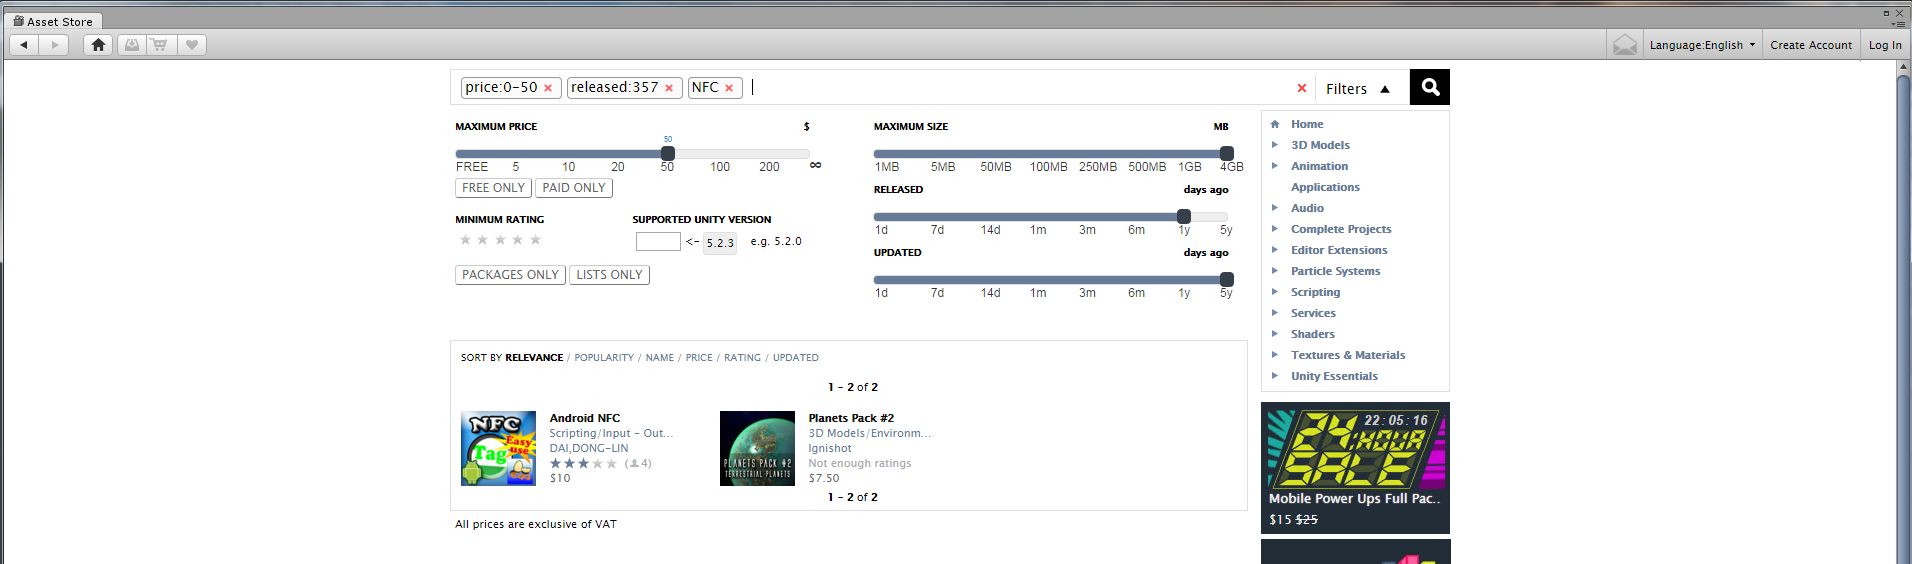
\includegraphics[width=10cm, height=5cm,keepaspectratio=true]{Importing4.png}
	\caption{Iskanje assetov}
\end{figure}
Vsak asset ima potem tudi opis kaj vsebuje, ceno, kakšne slike in mogoče tudi video implementacije ali primer projekta.\\
\begin{figure}[ht!]
	\centering
	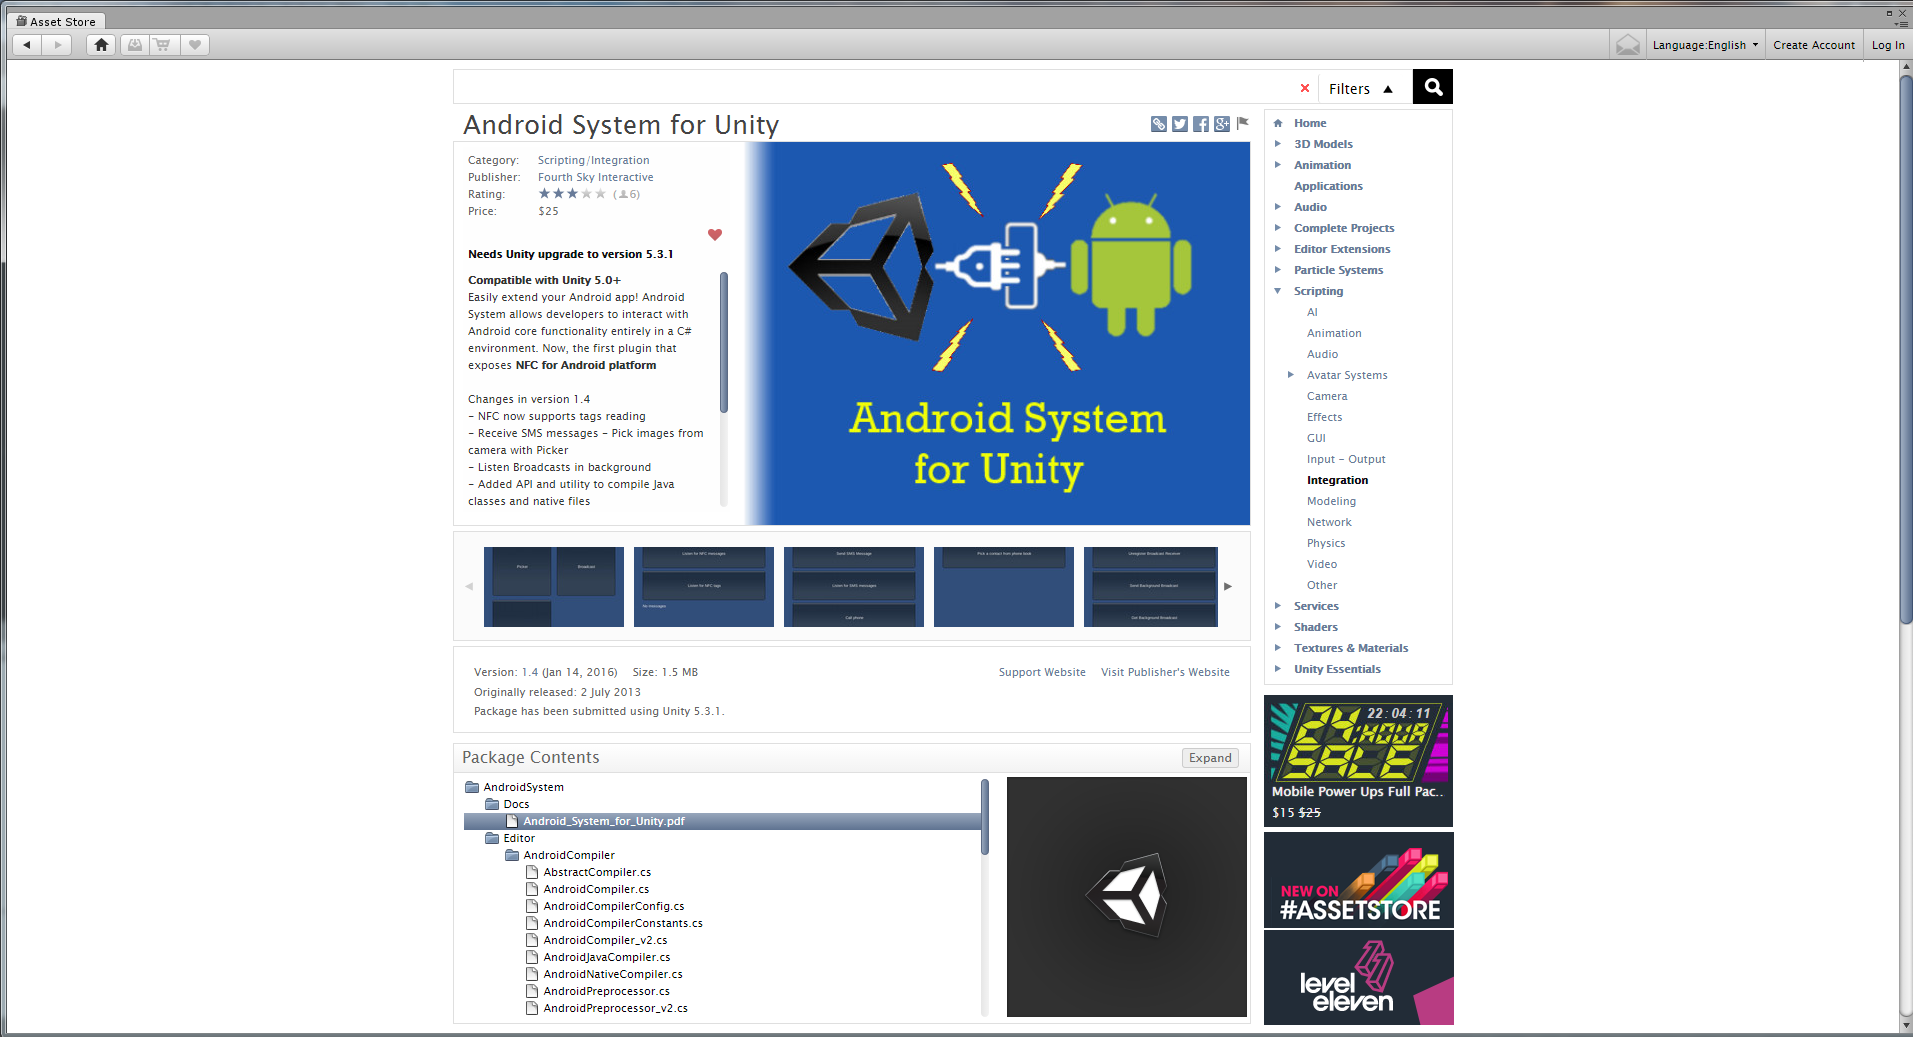
\includegraphics[width=10cm, height=10cm,keepaspectratio=true]{Importing5.png}
	\caption{Predstavitev asseta}
\end{figure}
Glavna prednost je da se zelo hitro vključijo v trenutni projekt in za njih ni potrebno spreminjati nastavitev. Razvijalec lahko tudi izbira katere stvari hoče prenesti v projekt in katere ne.\\
\begin{figure}[ht!]
	\centering
	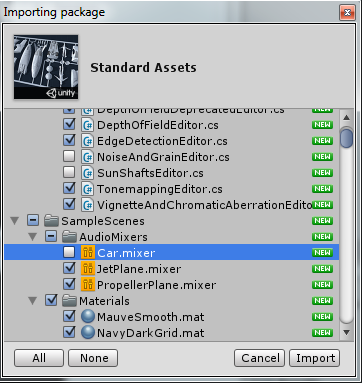
\includegraphics[width=10cm, height=10cm,keepaspectratio=true]{Importing6.png}
	\caption{Izbira kaj vključiti}
\end{figure}